\documentclass{kit}

\usepackage[ruled,vlined]{algorithm2e}
\SetAlgorithmName{}{}
% \SetAlgoCaptionSeparator{}

\author{Julius Vater - 2603322}
\title{Rechnerorganisation}
\begin{document}
\maketitle
\tableofcontents
\pagebreak
\section{Von-Neumann-Rechner}
  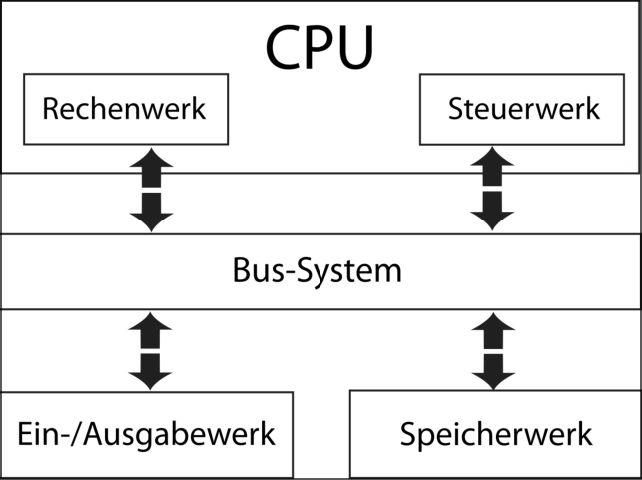
\includegraphics[width=\textwidth]{img/von_neumann.png}
  \begin{itemize}
    \item Steuerwerk
      \begin{itemize}
        \item Für die Abarbeitung des Programms zuständig
          \begin{itemize}
            \item Lädt den auszuführenden Befehl in das Befehlsregister (Holphase)
            \item Dekodiert den Befehl im Befehlsregister (Dekodierphase)
            \item Führt den dekodierten Befehl unter Verwendung der anderen CPU-Komponenten aus
              (Ausführungsphase)
          \end{itemize}
          Steuerregister beeinflussen Verhalten des Steuerwerks
      \end{itemize}
    \item Rechenwert
      \begin{itemize}
        \item ALU = "arithmetic logic unit"
        \item Führt auf Anweisung des Stuerewerks arithmetisch-logische Operationen aus
        \item Statusregister speichter zusätzliche Informationen über die letzte Berechnung, z.B.
          \begin{itemize}
            \item Negative Flag
            \item Carry Flag
            \item Overflow Flag
          \end{itemize}
      \end{itemize}
      \newpage
      \item Speicherwerk (Adresswerk)
        \begin{itemize}
          \item Regelt den Zugriff auf den Hauptspeicher, der Programme und Daten enthält
          \item Bei vielen modernen Prozessoren zusätzliche Aufgabenbereiche für MMU ("memory menagement
            unit") des Prozessors, z.B.
            \begin{itemize}
              \item Zugriffsschutz
              \item Segmentierung
              \item Paging (Kachelverwaltung)
            \end{itemize}
        \end{itemize}
      \item Registersatz
        \begin{itemize}
          \item Enthält die Register des Prozessors
          \item Spezialregister vs. allgemein verwendbare (general purpose) Register
        \end{itemize}
      \item Systembusschnittstelle
        \begin{itemize}
          \item Erlaubt dem Prozessor, über den Systembus mit anderen Rechnerkomponenten zu 
            kommunizieren
          \item Bestehend aus:
            \begin{itemize}
              \item Stuerbus (unidirektional / bidirektional): Hier gelangen Stuerinformationen
                von/zum Prozessor
              \item Adressbus (unidirektional): Leitungen, auf denen die Adressinformation
                transportiert wird
              \item Datenbus (bidirektional): Hier werden Daten und Befehle von/zum Prozessor 
                transportiert
            \end{itemize}
        \end{itemize}
  \end{itemize}
\section{MIMA}
  \begin{itemize}
    \item Mikroprogrammierte Minimalmaschine
    \item Sehr einfaches Modell für eine CPU mit Von-Neumann-Architektur
    \item Wurde im Rahmen der RO-Vorlesung entwickelt und wird dort vorgestellt
  \end{itemize}
  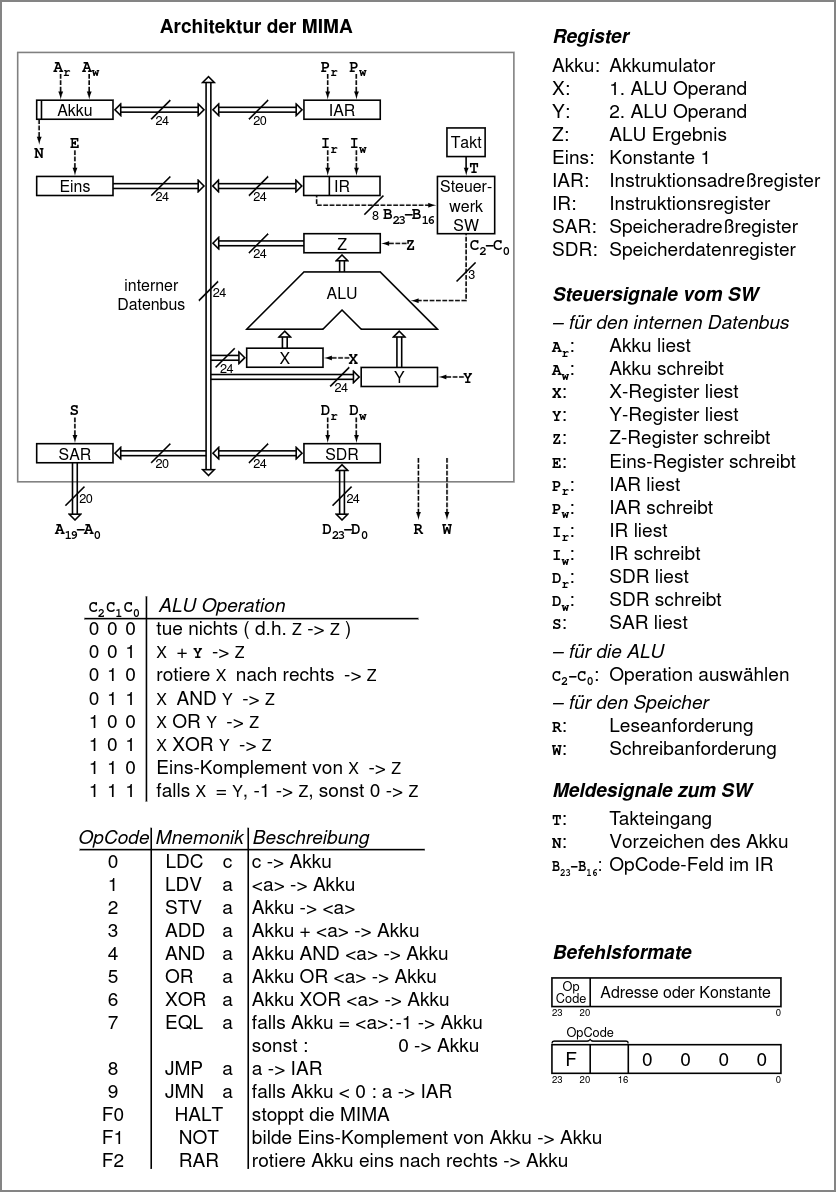
\includegraphics[width=\textwidth]{img/mima.png}
  \newpage
\section{Mikroprogrammierung}
  \begin{itemize}
    \item Das MIMA-Steuerwerk ist mikroprogrammiert
    \item Ein Maschinenbefehl wird durch ein kleines Programm von Mikrobefehlen ausgeführt
    \item Jeder dieser Mikrobefehle gibt an, welcher der Steuerleitungen in einem Taktzyklus aktiv sind
    \item Register-Transfer-Anweisungen als alternative Schreibweise:
      \begin{itemize}
        \item $A_w=1,P_r=1$ (Steuersignale)
        \item AKKU $\ra$ IAR (Register-Transfer)
      \end{itemize}
  \end{itemize}
\section{RISC-V}
  \begin{itemize}
    \item Folgt den Desingprinzipien einer RISC-Architektur (Reduced Instruction Set Computing)
    \item Register
      \begin{itemize}
        \item \$zero (0): enthält Null-Wert
        \item \$ra (1): Rücksprungadresse (für jal)
        \item \$sp (2): Stack Pointer
        \item \$gp (3): Global Pointer
        \item \$tp (4): Thread Pointer
        \item \$t0-\$t2 (5-7): Temporäre Variablen
        \item \$s0/\$fp (8): Langlebige Variablen/Frame Pointer
        \item \$s1 (9): Langlebige Variablen
        \item \$a0-\$a1 (10-11): Argumente/Rückgabe
        \item \$a2-\$a7 (12-17): Argumente
        \item \$s2-\$s11 (18-27): Langlebige Variablen 
        \item \$t3-\$t6 (28-31): Temporäre Variablen 
      \end{itemize}
    \item Befehlsformate
      \begin{itemize}
        \item Standard Befehlsformate sind 32 Bit lang
        \item R-Typ ("Register"): 7 Bit Opcode, 3x 5 Bit Register-Nummer, 7+3 Bit Funktions-Code
        \item I-Typ ("Immediate"): 7 Bit Opcode, 2x 5 Bit Register-Nummer, 12 Bit Immediate-Wert,
          3 Bit Funktions-Code
        \item S-Typ ("Store"): 7 Bit Opcode, 2x 5 Bit Register-Nummer, 7+5 Bit Immediate-Wert, 3 Bit 
          Funktions-Code
        \item SB-Typ ("bedinger Spring"): 7 Bit Opcode, 2x 5 Bit Register-Nummer, 7+5 Bit 
          Immediate-Wert, 3 Bit Funktions-Code
        \item UJ-Typ ("Jump"): 7 Bit Opcode, 20 Bit Offset, 5 Bit Rücksprungadresse
      \end{itemize}
    \item Pseudobefehle
      \begin{itemize}
        \item Erweiterung des Befehlssatzes, ohne dass sich die Komplexität des CPU-Designs erhöht
        \item Werden nicht (direkt) auf einen Maschinenbefehl abgebildes, sondern durch einen oder
          mehrere native Befehle ersetzt
      \end{itemize}
    \item Datenpfade mit Steuerung
      \begin{itemize}
        \item Ein Datenpfad für die RISC-V Architektur
          \begin{itemize}
            \item kombiniert die Elemente, die für die Ausführung der verschiedenen Befehlsklassen 
              erfordeerlich sind
            \item Führt die grundlegenden Befehle load / store, ALU Operationen und Verzweigungen aus
          \end{itemize}
        \item Steuersignale
          \begin{figure}[h]
            \centering
            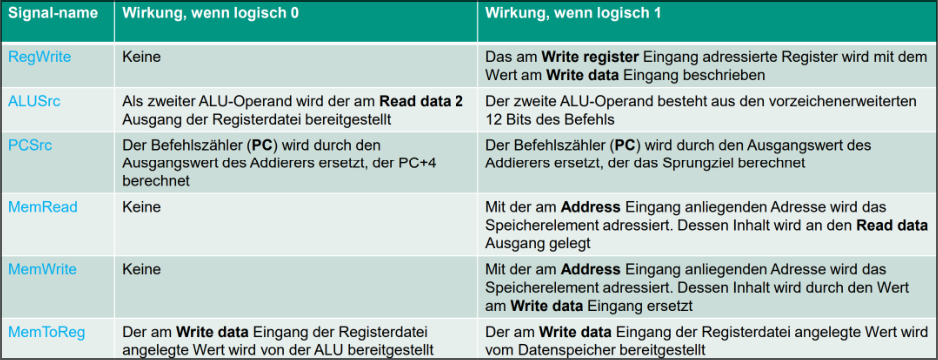
\includegraphics[width=\textwidth]{img/steuersignale.png}
          \end{figure}
      \end{itemize}
    \item Piplining
      \begin{itemize}
        \item Problemstellung
          \begin{itemize}
            \item Ziel: Reduzierung der Zeit in der CPU-Komponenten inaktiv sind
            \item Beobachtung: Datenbusarchitekturen bisher bekannter CPUs erlaubt größtenteils nur
              sequentielle Abarbeitung von Befehlen
            \item Folgerung: Gesucht wird eine Architektur, die die aktive Zeit aller CPU-Komponenten
              möglichst hoch hält
          \end{itemize}
        \item Vorteile
          \begin{itemize}
            \item Zeitdauer für die Abarbeitung eines Befehls wird nicht reduziert (tendentiell eher im
              Gegenteil)
            \item Aber: Pipelining erhöht den Durchsatz bei der Ausführung einer Befehlsfolge
            \item Im (theoretischen) Idealfall: Nach Befüllen der Pipeline wird jeden Takt die
              Ausführung eines Befehls abgeschlossen
            \item Maximal mögliche Taktfrequenz der Pipeline richtet sich nach der langsamsten 
              Pipeline-Stufe
          \end{itemize}
        \item Probleme
          \begin{itemize}
            \item Erhöhter Planungs- und Schaltungsaufwand
            \item Datenkonflikte: Daten werden benötigt, die noch nicht zur Verfügung stehen
            \item Kontrollflusskonflikte: Es ist nicht klar, welcher Befehl in die Pipeline geladen
              werden muss
            \item Resourcenkonflikte: Komponenten werden in mehr als einer Pipeline-Stufe benötigt
          \end{itemize}
        \item Durchsatz
          \begin{itemize}
            \item Durchsatz = Ausgeführte Befehle pro Benötigte Zeit
            \item Maßzahl für die Leistungsfähigkeit einer Mikroarchitektur (z.B. gemessen in  IPC,
              Instructions per Cycle
            \item Durchsatz erhöht sich durch Pipelining
            \item Im Idealfall
              \begin{itemize}
                \item k-stufige Pipeline mit n Befeheln: $n+(k-1)$ benötigte Taktzyklen
                \item Für $n\rai$: Durchsatz $\ra1$
              \end{itemize}
          \end{itemize}
        \item Speedup
          \begin{itemize}
            \item Speedup = Ohne Pipline benötigete Taktzyklen pro mit Pipeline benötigete Taktzyklen
            \item Geschwindigkeitsgewinn durch Einsatz von Pipelining
          \end{itemize}
      \end{itemize}
    \item RISC-V-Pipeline
      \begin{itemize}
        \item Stufen der RISC-V-Pipeline
          \begin{itemize}
            \item IF: Instruction Fetch
            \item ID: Instruction Decode
            \item EX: Execute
            \item MEM: Memory Access
            \item WB: Write Back
          \end{itemize}
        \item Abghänigkeiten
          \begin{itemize}
            \item Datenabhängigkeit: Zwei Instruktionen lesen/schreiben die selbe Datenresource
            \item Steuerabhängigkeit: Eine Instruktion bestimmt ob eine andere ausgeführt wird
            \item Strukturabhängigkeit: Zwei Instruktionen benötigen die selbe Resource
          \end{itemize}
        \item Typen von Datenabhängigkeiten
          \begin{itemize}
            \item Read after Write (RAW): Echte Datenabhängigkeit
            \item Write after Read (WAR): Gegenabhängigkeit
            \item Write after Write (WAW): Ausgabeabhängigkeit
          \end{itemize}
        \item Behandlung von Datenabhängigkeiten
          \begin{itemize}
              \item Software
                \begin{itemize}
                  \item Compiler erkennt Datenabhängigkeiten
                  \item Einfügen von NOP's verhindert das Auftreten von Konflikten
                  \item Umstrukturieren der Befehle statt NOP's falls möglich
                \end{itemize}
              \item Hardware
                \begin{itemize}
                  \item Guter Aufbau der Pipeline (Art und Anordnung der Stufen, Forwarding)
                  \item Sperren der Pipeline (pipeline interlock)
                \end{itemize}
          \end{itemize}
        \item Behandlung von Kontrollabhängigkeiten
          \begin{itemize}
            \item Software
              \begin{itemize}
                \item Compiler erkennt Kontrollabhängigkeiten
                \item Umordnen und Einfügen von NOP's
                \item Alternative: Kluges Assembler-Programmieren
              \end{itemize}
            \item Hardware
              \begin{itemize}
                \item Hardware erkennt Kontrollabhängigkeiten
                \item Sperren der Pipeline (pipeline interlock)
                \item Sprungvorhersagen
              \end{itemize}
          \end{itemize}
      \end{itemize}
  \end{itemize}
\section{Halbleiterspeichertypen}
  \subsection{Flüchtige Speichertypen}
    \begin{itemize}
      \item Flüchtiger (volatiler) Halbleiterspeicher: Verliert Inhalt, wenn Versorgungsspannung
      \item RAM: Random Access Memory (wahlfreier Zugriff auf alle Speicheradressen)
      \item Statischer RAM (SRAM)
        \begin{itemize}
          \item Speicherelemente sind Flipflops, die meist in CMOS-Technik aufgebaut sind
          \item Hohe Genauigkeit, hoher Preis pro Speichermenge
        \end{itemize}
      \item Dynamischer RAM (DRAM)
        \begin{itemize}
          \item Speicherelemente sind Kondensatoren
          \item Wegen Leckströmen periodisches Auffrischen (Refresh) notwendig
          \item Langsamer als SRAM, günstiger pro Speichermenge
        \end{itemize}
      \item Quasi-statischer RAM (iRAM)
        \begin{itemize}
          \item Dynamischer RAM, bei dem eine integrierte Schaltung den Refresh automatisch durchführt
            (i = integriert)
          \item Können von außen daher als statischer RAM angesehen werden
        \end{itemize}
    \end{itemize}
  \subsection{Nicht-flüchtige Speichertypen}
    \begin{itemize}
    \item Nicht-flüchtiger (persistenter) Halbleiterspeicher: Speichert Inhalt auch ohne 
      Versorgungsspannung
    \item ROM: Read-only Memory
    \item Maske-programmiertes ROM
      \begin{itemize}
        \item Wird bei der Fertigung (irreversibel) programmiert
        \item Daher nur für große Stückzaheln geeignet
      \end{itemize}
    \item Pgrammable ROM (PROM)
      \begin{itemize}
        \item Einmalig mit einem Programmiergerät programmierbar
      \end{itemize}
    \item Erasable Programmable ROM (EPROM)
      \begin{itemize}
        \item Kann mehrmals beschrieben werden
        \item Vor Wiederbeschreiben Löschung durch Beleuchtung mit UV-Licht
      \end{itemize}
    \item Electronic Erasable Programmable ROM (EEPROM)
      \begin{itemize}
        \item Kann mehrmals beschrieben werden
        \item Schreiben und Löschen erfolgt rein elektronisch, allerdings sehr langsam
      \end{itemize}
    \item Flash-EEPROM
      \begin{itemize}
        \item Elektronisch löschbar wie EEPROM, aber nicht byte, sondern blockweise
        \item Insgesamt sehr schnell (Löschen ist die langsamste Operation)
        \item Weit verbreitet: USB-Sticks, Handys, SSDs, usw.
      \end{itemize}
    \end{itemize}
\section{Cache-Strukturen}
  \subsection{Segmentierung}
    Vorteile:
    \begin{itemize}
      \item Logische Struktur wird abgebildet (Codesegment, Datensegment, ...)
      \item Keine interne Fragmentierung, Segmente können mit der passenden Größe erzeugt werden
    \end{itemize}
    Nachteile:
    \begin{itemize}
      \item Segmente können nur ganz oder gar nicht ausgelagert werden
      \item Externe Fragmentierung möglich
    \end{itemize}
  \subsection{Paging}
    Vorteile:
    \begin{itemize}
      \item Keine externe Fragmentierung, da alle Seiten gleich groß
      \item Kleine Seiten lassen sich leicht ein- und auslagern
    \end{itemize}
    Nachteile:
    \begin{itemize}
      \item Potentiell hohe Zahl von aufeinaderfolgenden Seitenfehlern
      \item Interne Fragmentierung, da nur Vielfaches der Seitengröße allokiert werden kann
    \end{itemize}
  \subsection{Rolle der CPU}
    \begin{itemize}
      \item Memory Managemant Unit (MMU) der CPU übernimmt die Übersetzung von virtuellen zu physischen
        Adressen
      \item Meist Beschleunigung der Adressübersetzung durch Translation Lookaside Buffer (TLB)
      \item Segment- bzw. Seitentabelle speichert benötigte Zuordnung
      \item Tabellenzugriff entweder eigenständig durch Hardware (z.B x86) oder mit OS-Unterstützung
        bei einem TLB-Miss (z.B. MIPS)
    \end{itemize}
  \subsection{Swapping}
    \begin{itemize}
      \item Seiten können bei Speicherknappheit auf Sekundärspeicher ausgelagert werden
      \item Ausgelagerte Seiten werden als ausgelagert markiert
      \item Bei einem page fault wird eine Behandlung des OS ausgeführt
        \begin{itemize}
          \item Betroffene Seiten ausgelagert? Schutzverletzung/ungültige Seite?
          \item Falls keine Kache frei: Eine Seite auslagern
          \item Ausgelagerte Seite zurück in den Speicher an eine freie Kachel laden
          \item Ausführung des fehlgeschlagenen Befehls wiederholen
        \end{itemize}
    \end{itemize}
  \subsection{Haptspeicheradresse}
    \begin{itemize}
      \item Offset = log(Blockgröße)
      \item Anzahl Cache Zeilen = Kapazität/Blockgröße
      \item Index Feld = log(Anzahl Sätze)
      \item Anzahl Sätze = Anzahl Cache Zeilen/Cache Organisation
      \item Gesamtgröße = Speicherplatz Daten + Tag Speicherplatz
    \end{itemize}
  \subsection{Wann erfolg ein Write-Back?}
    Ein Write-Back erfolgt genau dann, wenn:
    \begin{itemize}
      \item Das \textbf{Write-Back-Verfahren} (nicht Write-Through) verwendet wird
      \item Ein \textbf{Cache Miss} bei einem Read- oder Write-Zugriff auftritt
      \item Für die betroffene Cache-Zeile gilt:
        \begin{itemize}
          \item Valid Bit = 1
          \item Dirty Bit = 1
        \end{itemize}
    \end{itemize}
    \textbf{Folge:} Der geänderte Block wird in den Hauptspeicher zurückgeschrieben.
  \subsection{Verhalten bei Cache Miss}
    \begin{itemize}
      \item Cache Miss + Write: Dirty Bit wird auf 1 gesetzt
      \item Cache Miss + Read: Dirty Bit wird auf 0 gesetzt
    \end{itemize}
  \subsection{Cache Hit vs. Cache Miss}
    Cache Hit:
    \begin{itemize}
      \item Der gespeicherte \textbf{Tag} stimmt mit dem tag der angeforderten Adresse überein
      \item Die Zeile/Seitennummer refernziert den korrekten Cache-Eintrag
      \item $\Rightarrow$ Zugriff erfolgt direkt aus dem Cache
    \end{itemize}
    Cache Miss:
    \begin{itemize}
      \item Der gespeicherte \textbf{Tag} stimmt \textbf{nicht} mit dem Tag der angeforderten Adresse
        überein
      \item Die Zeile enthält nicht die gewünschte Adresse
      \item $\Rightarrow$ Der entsprechende Block wird aus dem Hauptspeicher geladen
      \item $\Rightarrow$ Neuer Tag wird in den Cache eingetragen
    \end{itemize}
\section{Ein-/Ausgabe in Rechnersystemen}
  \subsection{Polling vs. Interrupt-gesteuerte I/O}
    Polling:
    \begin{itemize}
      \item CPU fragt regelmäßig den Gerätestatus ab
      \item Aktives Warten (busy waiting)
      \item Hohe CPU-Auslastung
    \end{itemize}
    Interrupt-gesteuerte I/O:
    \begin{itemize}
      \item Gerät signalisiert Ereignis per Interrupt
      \item CPU kann andere Aufgaben ausführen
      \item Geringe CPU-Belastung
    \end{itemize}
  \subsection{Programmed I/O}
    \begin{itemize}
      \item CPU steuert die gesamte Datenübertragung selbst
      \item Ablauf:
        \begin{itemize}
          \item Abfrage des Gerätestatus
          \item Datenübertragung Wort für Wort
        \end{itemize}
      \item Nachteil:
        \begin{itemize}
          \item CPU während der Übertragung blockiert
          \item Geringe Effizienz bei großen Datenmengen
        \end{itemize}
    \end{itemize}
  \subsection{Directe Memory Access (DMA)}
    \begin{itemize}
      \item DMA-Controller übernimmt die Datenübertragung
      \item CPU initialisiert DMA und wird danach entlastet
      \item Vorteile:
        \begin{itemize}
          \item Sehr geringe CPU-Belastung
          \item Hohe Übertragungsgeschwindigkeit
          \item Geeignet für große Datenmengen
        \end{itemize}
    \end{itemize}
\end{document}
